\begin{flushleft}
Il seguente script organizza il risultato dell'esercizio per fare il plot dei confronti:
\lstinputlisting[language=matlab]{cap_4/es5/es5.m}
\begin{figure}[H]
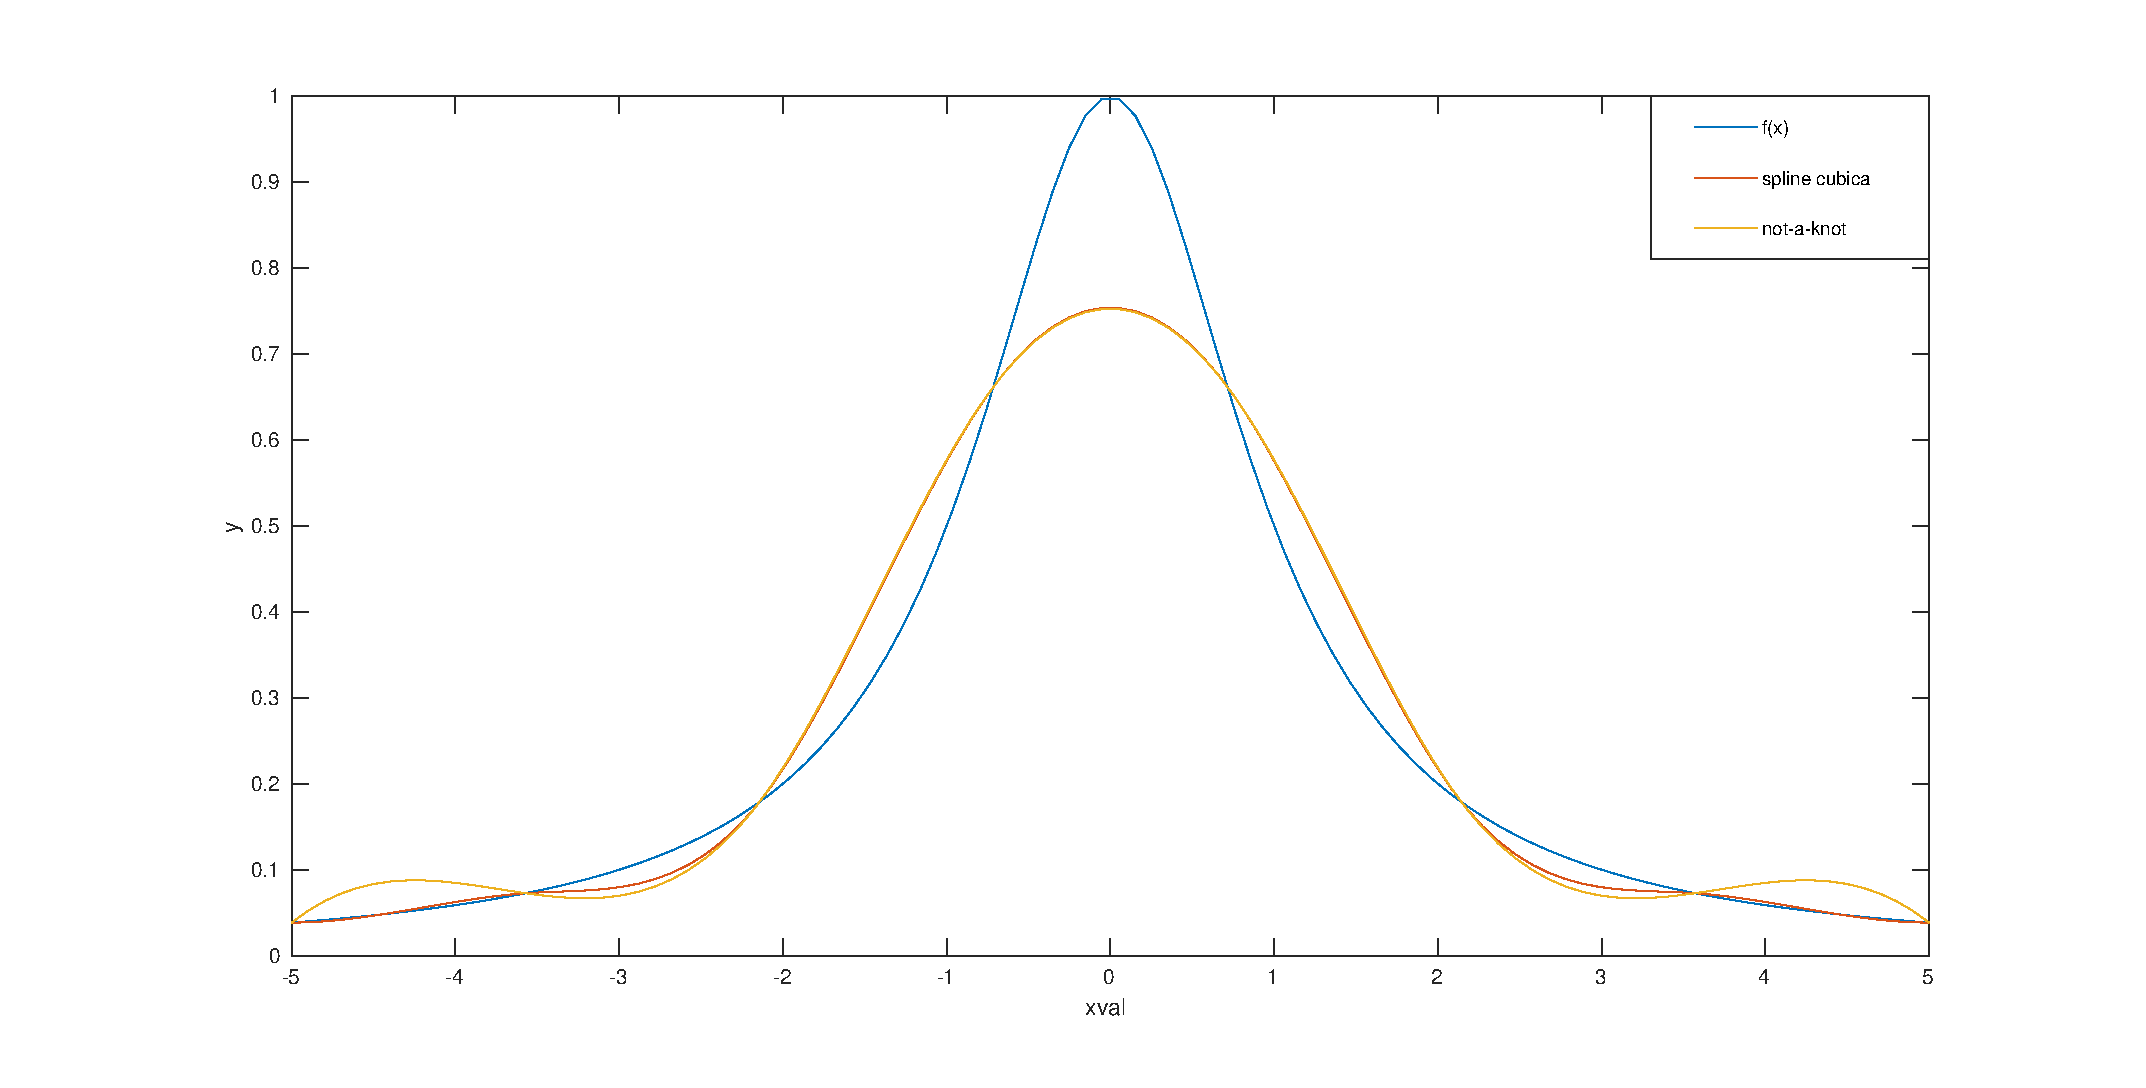
\includegraphics[width=480px, height=280px]{plot/fes45b.eps}
\caption{\texttt{Confronto tra spline e funzione reale}}
\end{figure}
\begin{figure}[H]
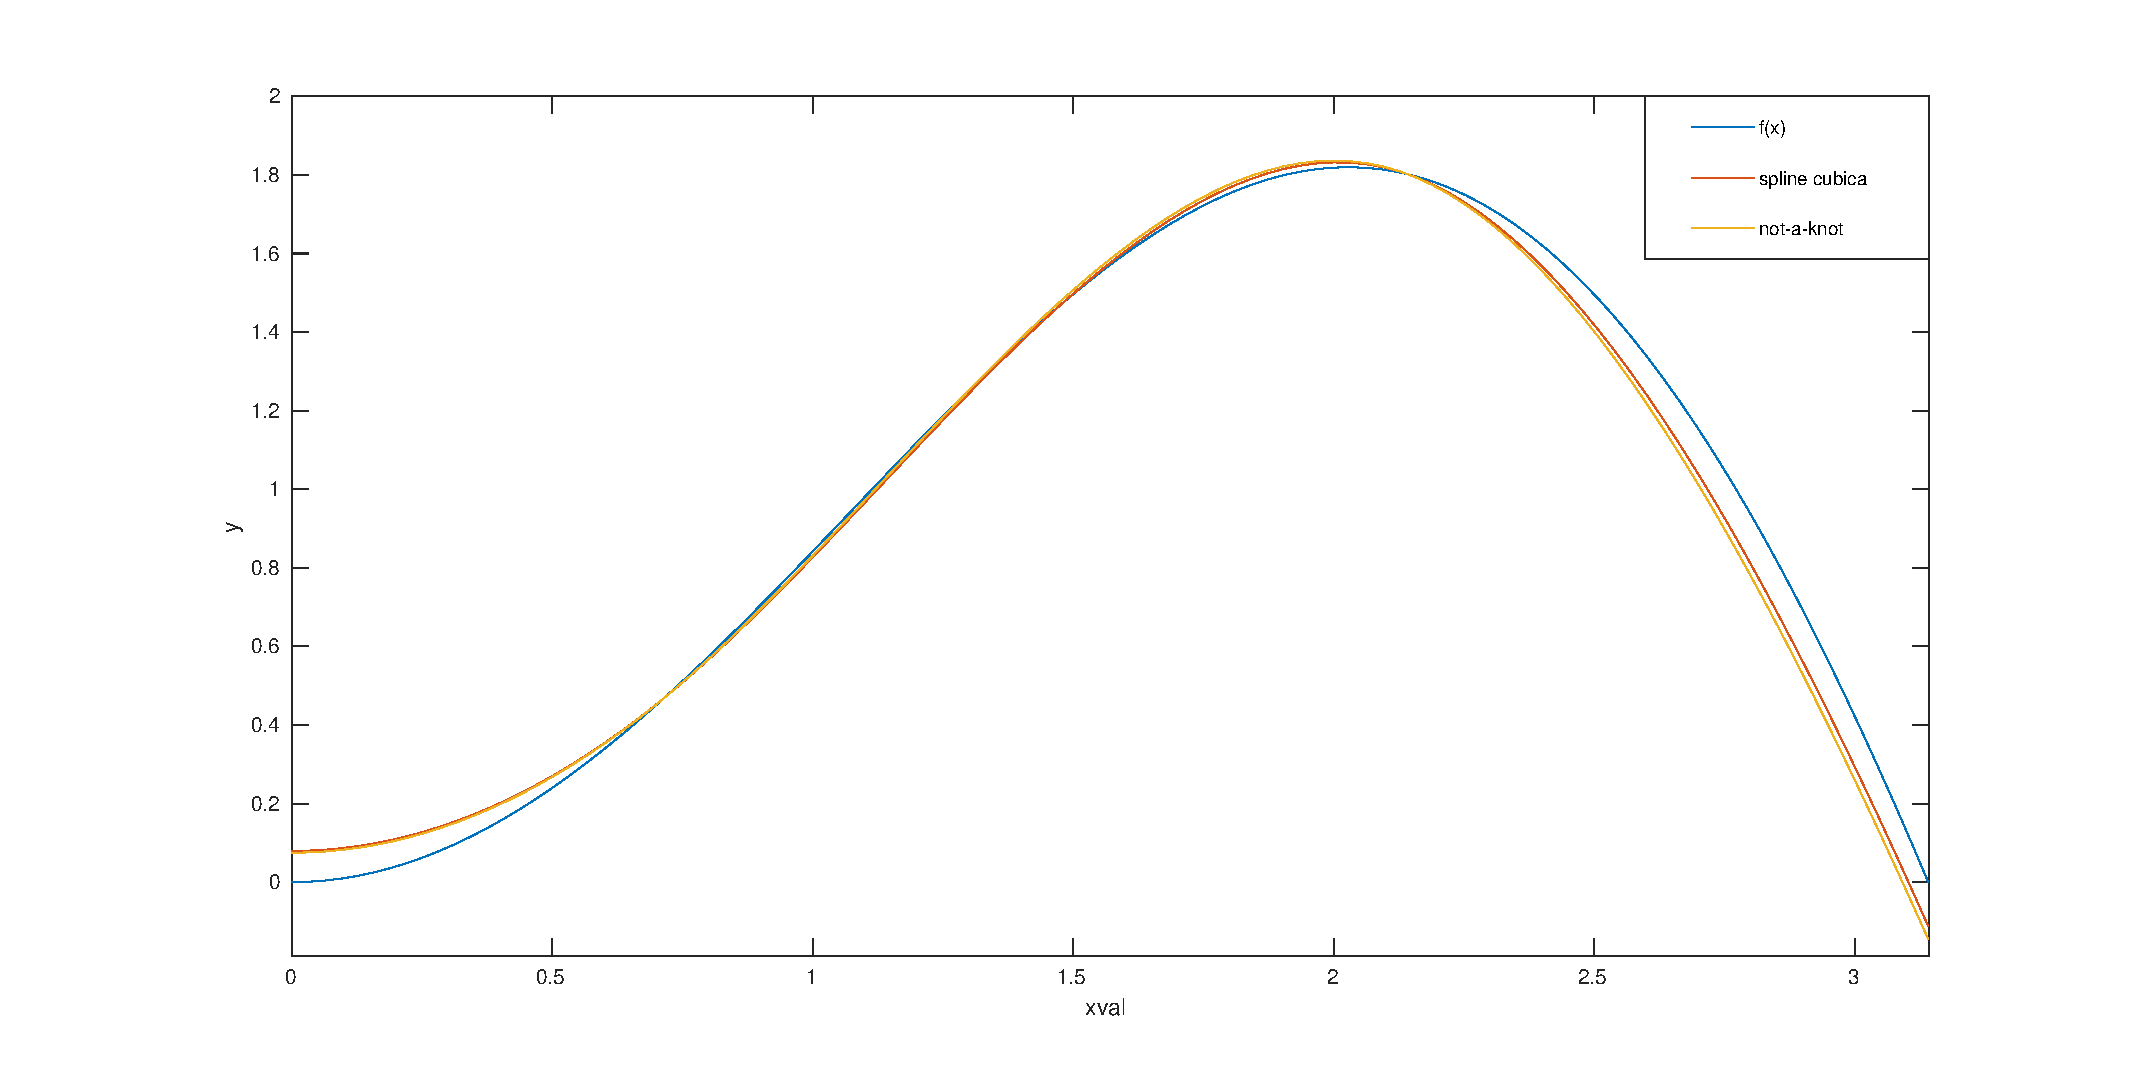
\includegraphics[width=480px, height=280px]{plot/fes45a.eps}
\caption{\texttt{Confronto tra spline e funzione reale}}
\end{figure}
\end{flushleft}